\documentclass[letterpaper,12pt]{article}\usepackage[]{graphicx}\usepackage[]{color}
%% maxwidth is the original width if it is less than linewidth
%% otherwise use linewidth (to make sure the graphics do not exceed the margin)
\makeatletter
\def\maxwidth{ %
  \ifdim\Gin@nat@width>\linewidth
    \linewidth
  \else
    \Gin@nat@width
  \fi
}
\makeatother

\definecolor{fgcolor}{rgb}{0.345, 0.345, 0.345}
\newcommand{\hlnum}[1]{\textcolor[rgb]{0.686,0.059,0.569}{#1}}%
\newcommand{\hlstr}[1]{\textcolor[rgb]{0.192,0.494,0.8}{#1}}%
\newcommand{\hlcom}[1]{\textcolor[rgb]{0.678,0.584,0.686}{\textit{#1}}}%
\newcommand{\hlopt}[1]{\textcolor[rgb]{0,0,0}{#1}}%
\newcommand{\hlstd}[1]{\textcolor[rgb]{0.345,0.345,0.345}{#1}}%
\newcommand{\hlkwa}[1]{\textcolor[rgb]{0.161,0.373,0.58}{\textbf{#1}}}%
\newcommand{\hlkwb}[1]{\textcolor[rgb]{0.69,0.353,0.396}{#1}}%
\newcommand{\hlkwc}[1]{\textcolor[rgb]{0.333,0.667,0.333}{#1}}%
\newcommand{\hlkwd}[1]{\textcolor[rgb]{0.737,0.353,0.396}{\textbf{#1}}}%

\usepackage{framed}
\makeatletter
\newenvironment{kframe}{%
 \def\at@end@of@kframe{}%
 \ifinner\ifhmode%
  \def\at@end@of@kframe{\end{minipage}}%
  \begin{minipage}{\columnwidth}%
 \fi\fi%
 \def\FrameCommand##1{\hskip\@totalleftmargin \hskip-\fboxsep
 \colorbox{shadecolor}{##1}\hskip-\fboxsep
     % There is no \\@totalrightmargin, so:
     \hskip-\linewidth \hskip-\@totalleftmargin \hskip\columnwidth}%
 \MakeFramed {\advance\hsize-\width
   \@totalleftmargin\z@ \linewidth\hsize
   \@setminipage}}%
 {\par\unskip\endMakeFramed%
 \at@end@of@kframe}
\makeatother

\definecolor{shadecolor}{rgb}{.97, .97, .97}
\definecolor{messagecolor}{rgb}{0, 0, 0}
\definecolor{warningcolor}{rgb}{1, 0, 1}
\definecolor{errorcolor}{rgb}{1, 0, 0}
\newenvironment{knitrout}{}{} % an empty environment to be redefined in TeX

\usepackage{alltt}
\usepackage[top=1in,bottom=1in,left=1in,right=1in]{geometry}
\usepackage{setspace}
\usepackage[colorlinks=true,urlcolor=blue,citecolor=blue,linkcolor=blue]{hyperref}
\usepackage{indentfirst}
\usepackage{multirow}
\usepackage{booktabs}
\usepackage[final]{animate}
\usepackage{graphicx}
\usepackage{verbatim}
\usepackage{rotating}
\usepackage{tabularx}
\usepackage{array}
\usepackage{subfig} 
\usepackage[noae]{Sweave}
\usepackage{cleveref}
\usepackage[figureposition=bottom]{caption}
\usepackage{paralist}
\usepackage{acronym}
\usepackage{outlines}
\usepackage{pdflscape}

% knitr options and libs


\setlength{\parskip}{\baselineskip}
\setlength{\parindent}{0pt}
\IfFileExists{upquote.sty}{\usepackage{upquote}}{}
\begin{document}

The following summarizes a brief analysis to estimate changes in dissolved oxygen along a tidal cycle.  Estimates were from CTD vertical profiles of dissolved oxygen on the longitudinal axis of Escambia Bay and ADCP data of water direction and velocities at P05.  
\begin{enumerate}
\item{
CTD data from July 23rd, 2014 were used to estimate the horizontal gradient in dissolved oxygen.


{\centering 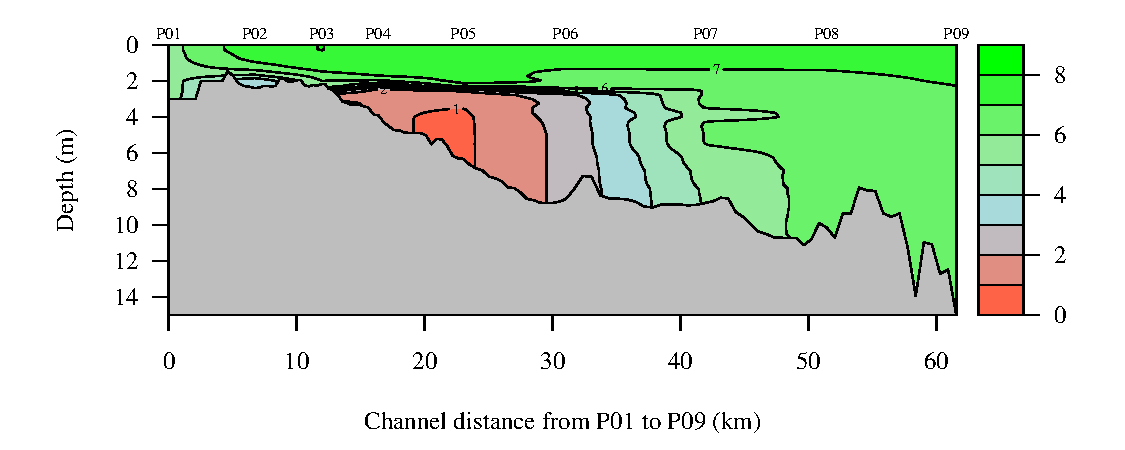
\includegraphics[width=\textwidth]{figs/unnamed-chunk-1-1} 

}



}
\item{
ADCP data at P05 for the month of July were used to estimate the average tidal excursion per tidal cycle.  The ADCP data were first reprocessed from the raw data by averaging the north and south vectors for the lowest three bins, finding the first principal component from the averaged vector, and reprojecting the averaged vector along the first principal component.  


The plot shows distance travelled of a theoretical water parcel within a one-month period centered on July 23\textsuperscript{rd}.  The colors mark changes in tidal direction.  Average distance traveled was 3.05 km for landward excursions (blue) and 2.37 km for seaward excursions (red).


{\centering 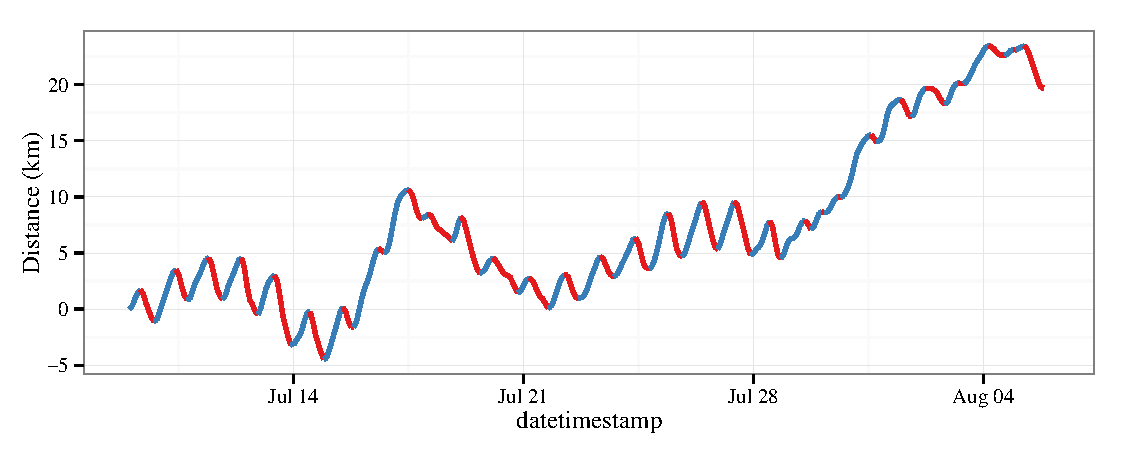
\includegraphics[width=\maxwidth]{figs/unnamed-chunk-3-1} 

}



}
\item{

The bottom-water dissolved oxygen gradient at P05 was estimated from the CTD data using the average distance travelled within a tidal cycle.  The average distance travelled during a landward or seaward flowing tide was plotted on interpolated bottom-water dissolved oxygen to estimate the DO gradient in each direction, relative to P05.  The estimated gradient was 0.88 mg/L for landward flow (DO change in blue) and 0.16 mg/L for seaward flow (DO change in red).  For both cases, dissolved oxygen was higher as distance increased from P05.  


{\centering 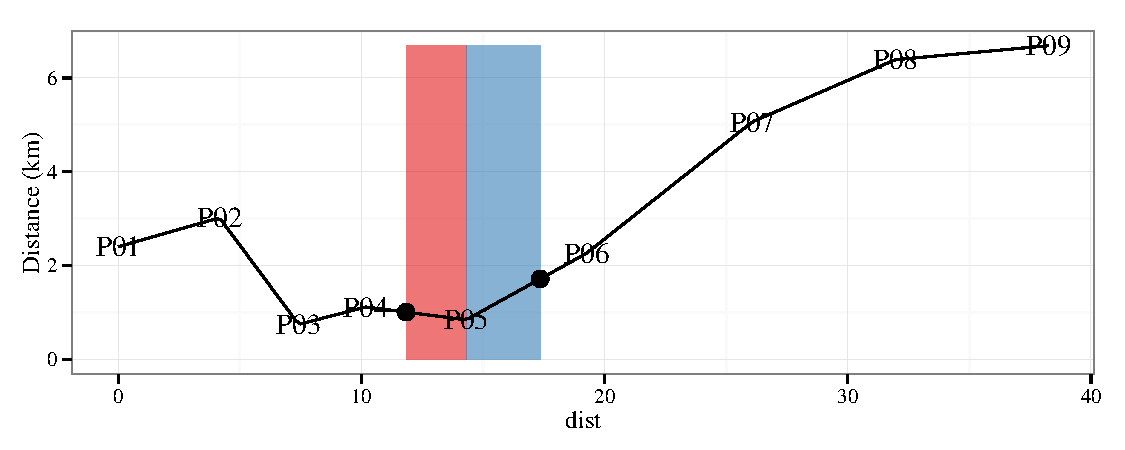
\includegraphics[width=\maxwidth]{figs/unnamed-chunk-5-1} 

}



}
\item{
Finally, a rate of oxygen change per tidal cycle was estimated.  The average time for each tidal cycle was estimated such that a unit of time could be assigned to each estimate from the previous step.  On average, the time for landward flow in the bottom was 12.45 hours and the time for seaward flow was 9.16 hours. This means that the rate of landward flow of dissolved oxygen was 0.07 mg/L/hr and the rate of seaward flow of dissolved oxygen was  mg/L/hr.
}
\item{
This exercise was repeated for each CTD date to estimate rate of DO change with each tidal cycle.  CTD dates with a corresponding complete record of ADCP data within one month were used.


{\centering 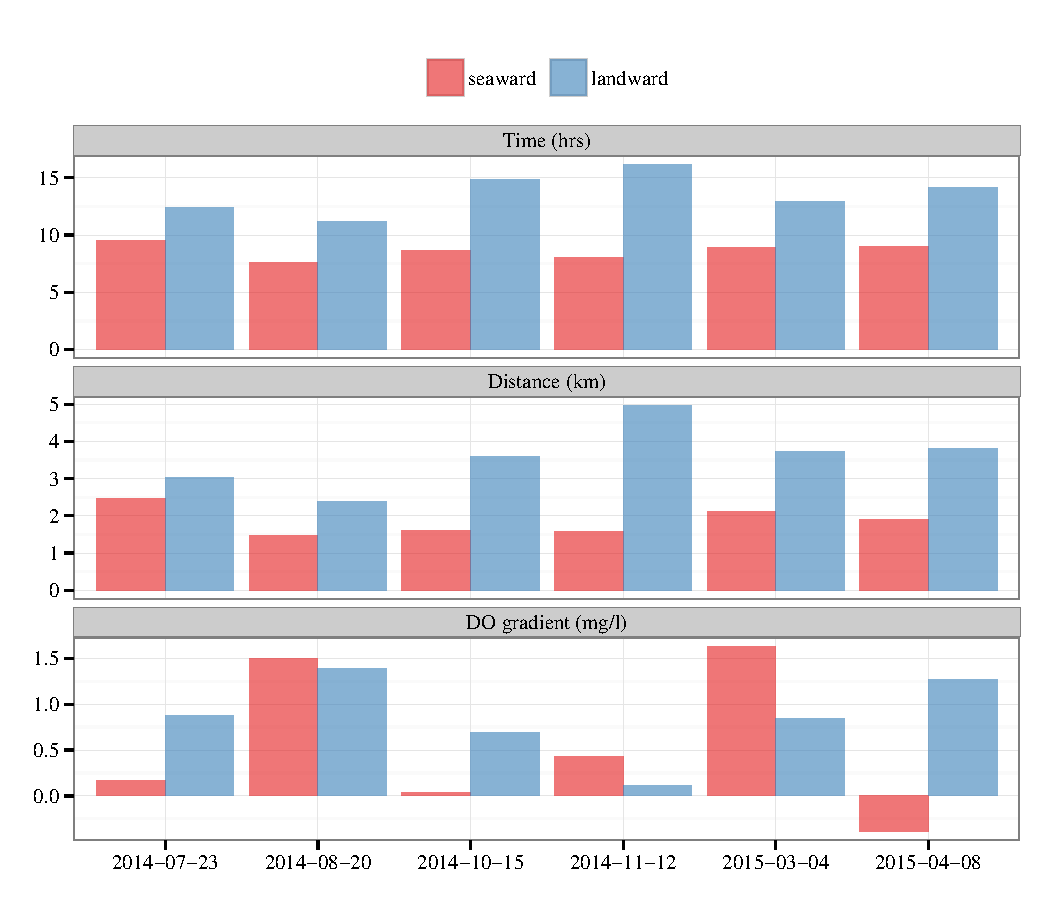
\includegraphics[width=\maxwidth]{figs/unnamed-chunk-6-1} 

}




}
\item{
CTD plots for each selected date in the previous plot, only first four


{\centering 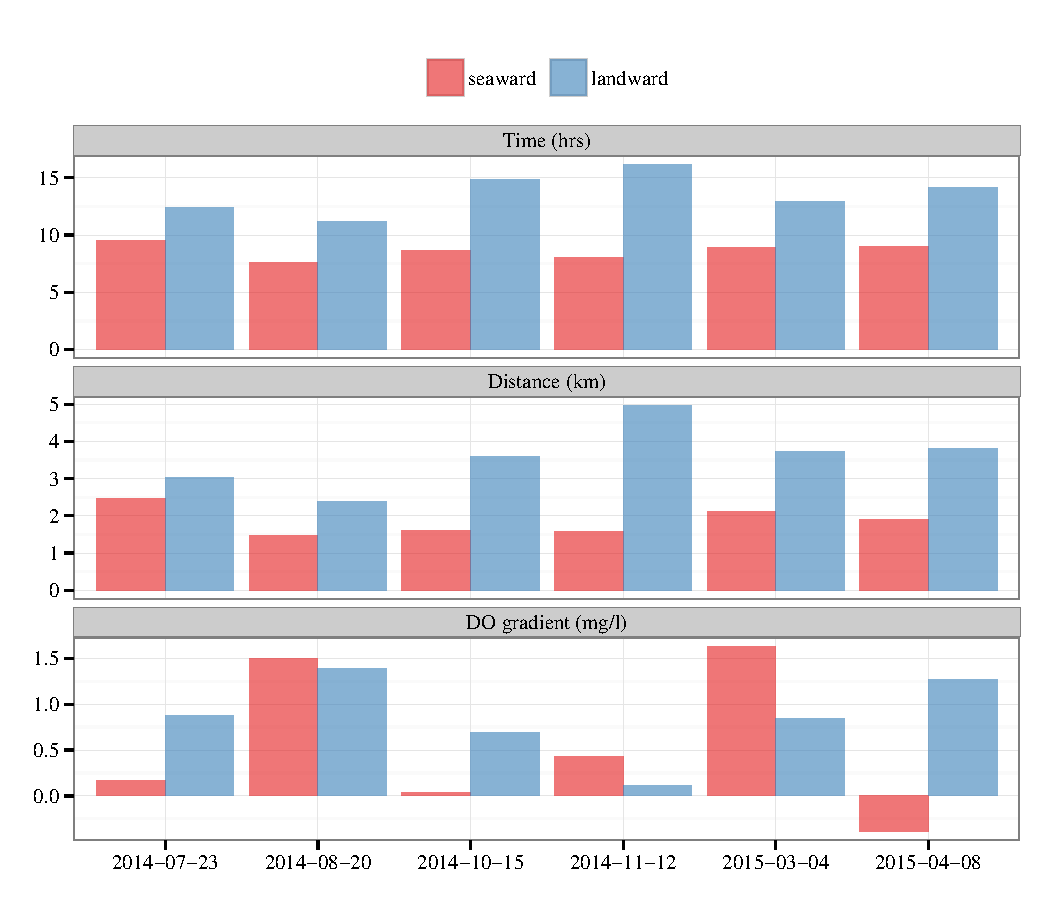
\includegraphics[width=\maxwidth]{figs/unnamed-chunk-7-1} 

}



}
\item{
Tidal excursion plots and graphical illustration of bottom-water DO gradient for the first four dates in the bar plot. 


{\centering 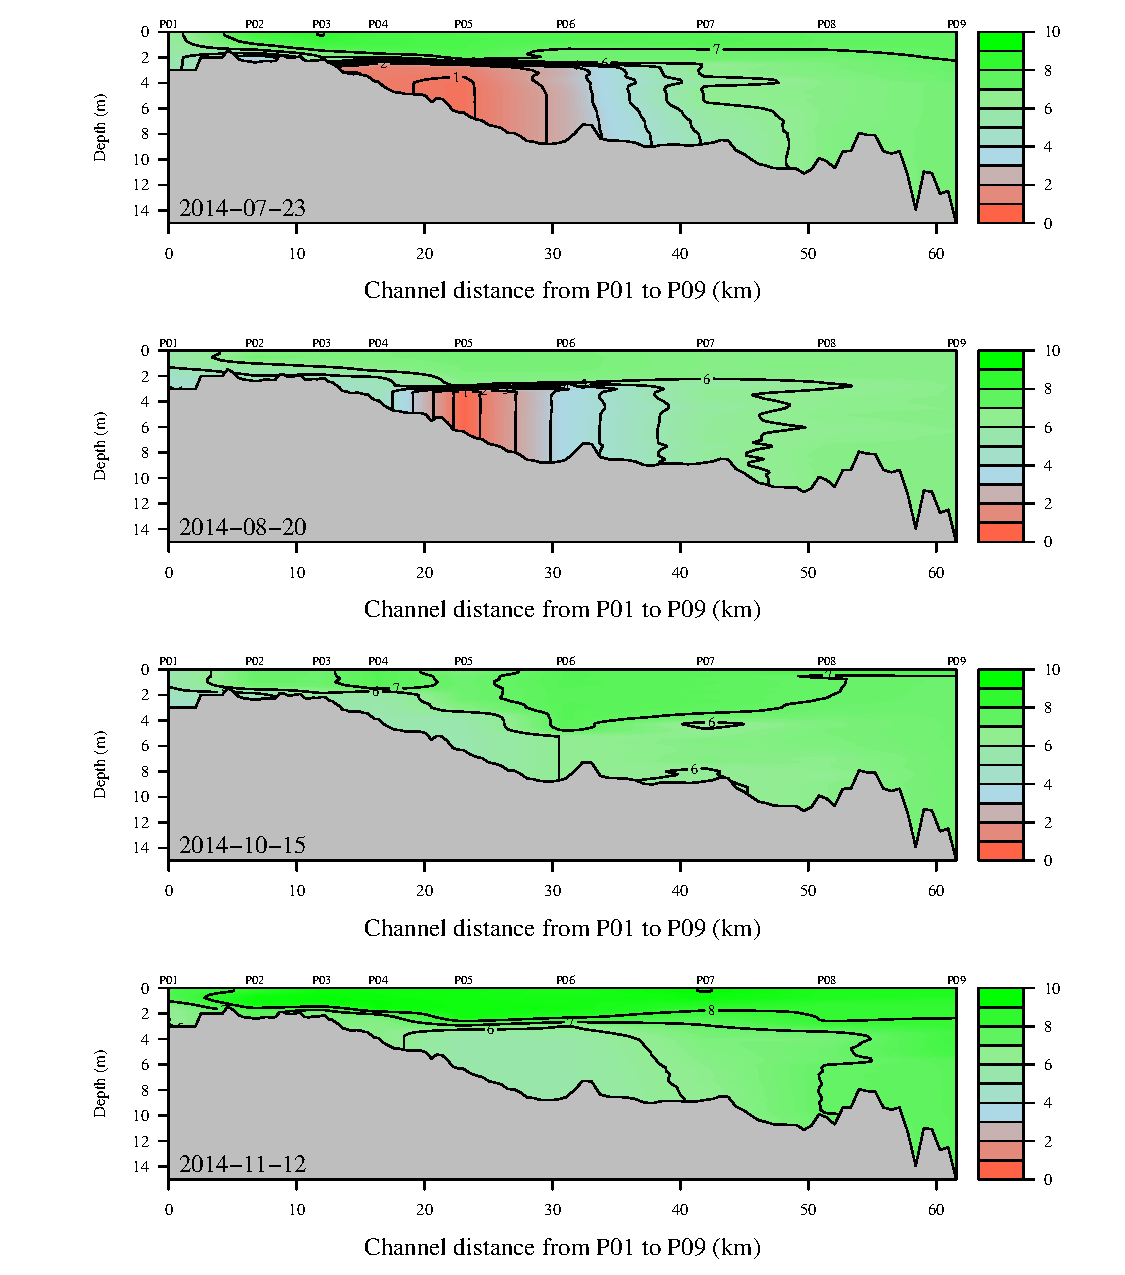
\includegraphics[width=\textwidth]{figs/unnamed-chunk-8-1} 

}




}
\end{enumerate}

\end{document}
